\section{Aufgabe 12}
\subsection{a)}
Mittelwerte:
\begin{equation*}
  \vec{\mu}_0 = \begin{pmatrix}
                  -0,027\\
                   2,980\\
  \end{pmatrix}
\end{equation*}
\begin{equation*}
  \vec{\mu}_1 = \begin{pmatrix}
                   5,986\\
                   3,085\\
  \end{pmatrix}
\end{equation*}

\subsection{b)}
Kovarianzmatrizen:
\begin{equation*}
  V_0 = \begin{pmatrix}
                  12,209 &  8,158 \\
                  8,158  &  6,7223 \\
  \end{pmatrix}
\end{equation*}
\begin{equation*}
  V_1 = \begin{pmatrix}
                  12,352 &  7,411 \\
                  7,411 &  5,477 \\
  \end{pmatrix}
\end{equation*}

Kombinierte Kovaranzmatrix:
\begin{equation*}
  V_{\symup{0,1}} = \begin{pmatrix}
                  21,322 &  7,943 \\
                  7,943 &  6,103 \\
  \end{pmatrix}
\end{equation*}

\subsection{c)}
Zu Berechnung der Fisher-Diskriminante, müssen zunächst die Streumatrizen berechnet werden:
\begin{equation*}
  S_0 = \begin{pmatrix}
                  122077,077 & 81575,940 \\
                  81575,940 & 67221,910 \\
  \end{pmatrix}
\end{equation*}
\begin{equation*}
  S_1 = \begin{pmatrix}
                  123509.502 & 74100.151 \\
                  74100.151 & 54767.673 \\
  \end{pmatrix}
\end{equation*}

Daraus wird die Gesamtstreuung $S_W$ berechnet
\begin{equation*}
  S_W = S_0 + S_1= \begin{pmatrix}
                  245586,579 & 155676,091 \\
                  155676,091 & 121989,583 \\
  \end{pmatrix}
\end{equation*}
Die Fisher-Diskriminante lässt sich nun mit Hilfe der Formel
\begin{equation}
  \vec{\lambda} = S_W^{-1} (\vec{\mu_0} - \vec{\mu_1})
\end{equation}
berechnen:
\begin{equation*}
  \vec{\lambda} = \begin{pmatrix}
                  -0,0001253 \\
                  0,00015904 \\
  \end{pmatrix}
\end{equation*}
Diese lässt sich als Geradengleichung der Form $\vec{\lambda} = \lambda \cdot \vec{e}_{\lambda}$  darstellen:, mit
\begin{equation*}
  \lambda = 0,00020247
\end{equation*}
und
\begin{equation}
  \label{Einheitsvektor}
  \vec{e}_{\lambda} = \begin{pmatrix}
                  -0,619 \\
                  0,785 \\
  \end{pmatrix}
\end{equation}
Der Einheitsvektor \eqref{Einheitsvektor} lässt sich für die Projektion in den nächsten Aufgabenteilen verwenden.

\subsection{d)}
Zu Projektion der einzelnen Punkte auf die Gerade $\vec{\lambda}$ wird folgende Formel verwendet:
\begin{equation*}
  P_{\symup{\lambda}}(\vec{x}) = ( \vec{x} \cdot \vec{e}_{\lambda} ) \cdot \vec{e}_{\lambda}
\end{equation*}
wobei für die eindimensionale Verteilung nur der Betrag genommen wird, also nur $(\vec{x}\cdot \vec{e}_{\lambda})$.
Die eindimensionale Verteilung auf der Geraden ist in Abbildung \ref{abb:1} zu sehen.

\begin{figure}
  \centering
  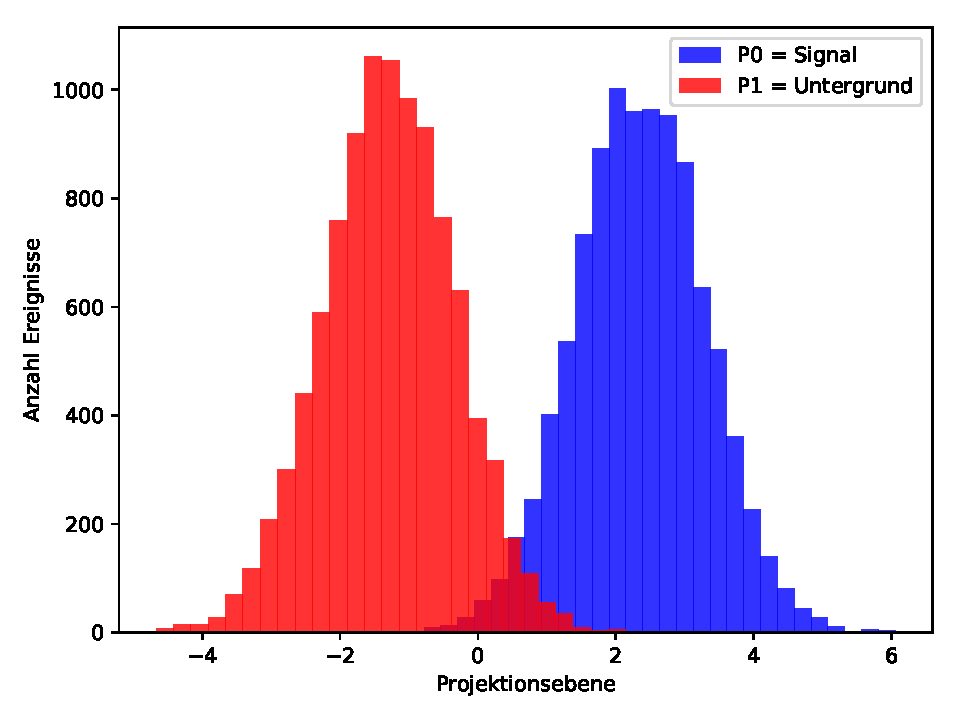
\includegraphics[scale=0.7]{Aufgabe12/Projektionen.pdf}
  \caption{Projektion auf die Gerade.}
  \label{abb:1}
\end{figure}

\subsection{e)}
Die Effizienz wird mit der Formel:
\begin{equation*}
  \symup{Effizienz} = \frac{t_p}{t_p + f_p}
\end{equation*}
berechnet und die Reinheit mir:
\begin{equation}
  \symup{Reinheit} = \frac{t_p}{t_p + f_n}
\end{equation}
Die Effizienz und die Reinheit in Abhängigkeit der Cut-Stelle $\lambda_{\symup{cut}}$ ist in Abbildung
\ref{abb:2} dargestellt.
\begin{figure}
  \centering
  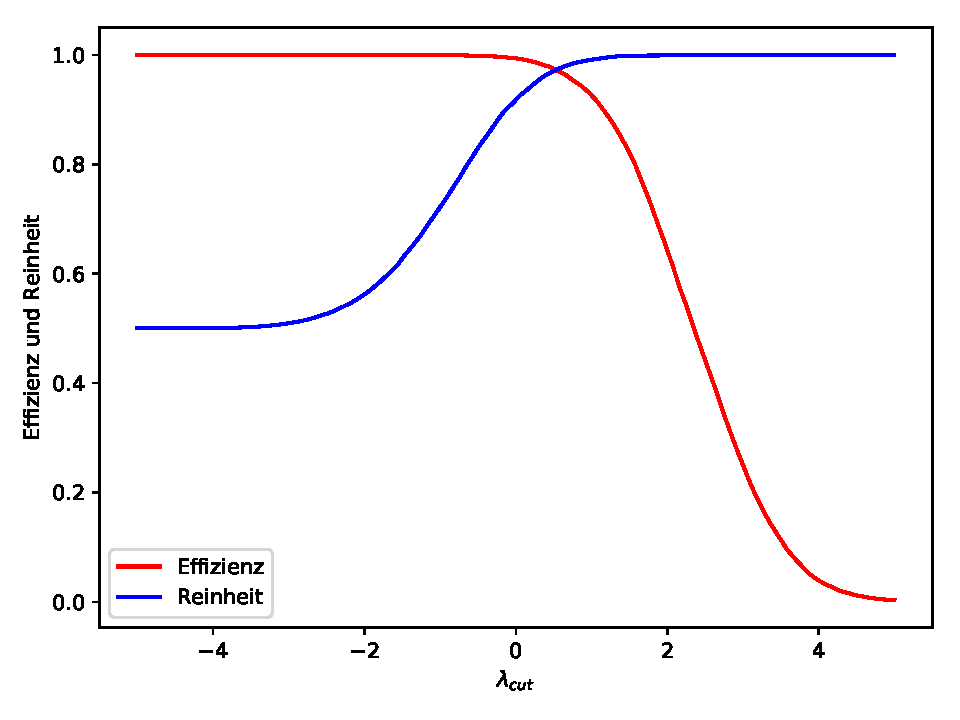
\includegraphics[scale=0.7]{Aufgabe12/EffizienzReinheit.pdf}
  \caption{Effizienz und Reinheit in Abhängigkeit der Cut-Stelle.}
  \label{abb:2}
\end{figure}

\subsection{f)}
Das Verhältnis zwischen Signal und Untergrund in Abhängigkeit von $\lambda_{\symup{cut}}$
ist in Abbildung \ref{abb:3} zu sehen. Der Maximalwert liegt hier bei
\begin{equation*}
  \lambda_{\symup{cut,Verhältnis}} \approx 2,17
\end{equation*}
\begin{figure}
  \centering
  \includegraphics[scale=0.7]{Aufgabe12/Verhältnis.pdf}
  \caption{Verhältnis S/B in Abhängigkeit der Cut-Stelle.}
  \label{abb:3}
\end{figure}

\subsection{g)}
Die Signifikanz $\frac{S}{\sqrt{S+B}} $ in Abhängigkeit von $\lambda_{\symup{cut}}$ ist in Abbildung
\ref{abb:4} dargestellt.
Der Maximalwert liegt hier bei:
\begin{equation*}
  \lambda_{\symup{cut, Signifikanz}} \approx 0,45
\end{equation*}
\begin{figure}
  \centering
  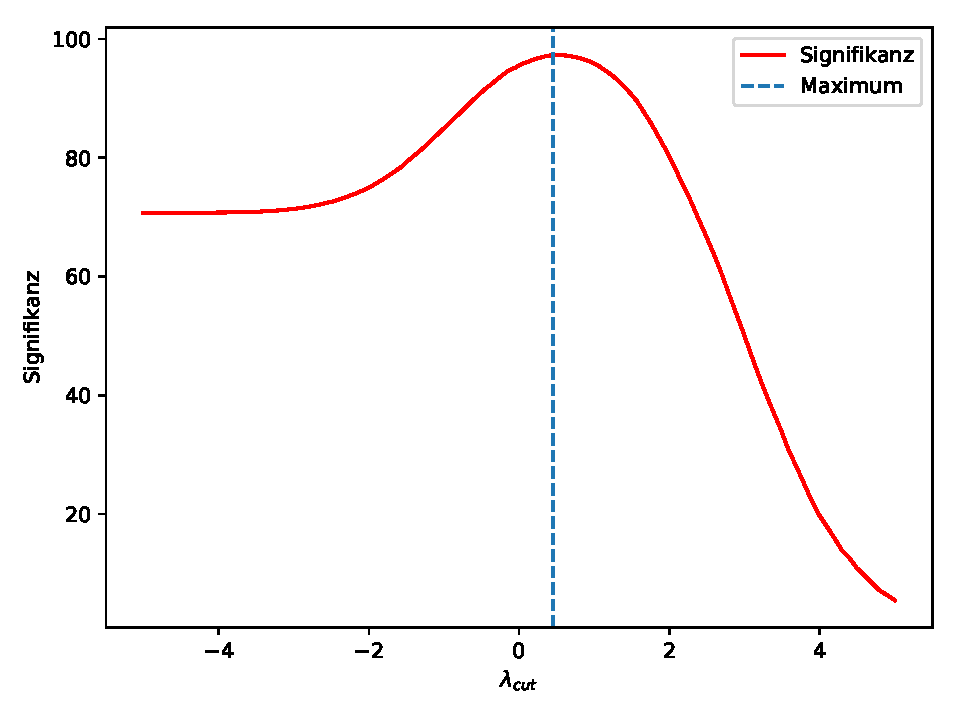
\includegraphics[scale=0.7]{Aufgabe12/Signifikanz.pdf}
  \caption{Signifikanz in Abhängigkeit der Cut-Stelle.}
  \label{abb:4}
\end{figure}

\subsection{f)}
Das ganze soll nun mit einem anderen Signal erneut untersucht werden:

Mittelwert:
\begin{equation*}
  \vec{\mu}_2 = \begin{pmatrix}
                  -0,0958\\
                   2,8788\\
  \end{pmatrix}
\end{equation*}

Kovarianzmatrix:
\begin{equation*}
  V_2 = \begin{pmatrix}
                  12,236 &  8,160 \\
                  8,160 &  6,758 \\
  \end{pmatrix}
\end{equation*}

Kombinierte Kovaranzmatrix:
\begin{equation*}
  V_{\symup{2,1}} = \begin{pmatrix}
                  15,398 &  7,582 \\
                  7,582 &  5,597 \\
  \end{pmatrix}
\end{equation*}

Streumatrix:
\begin{equation*}
  S_2 = \begin{pmatrix}
                  12223,886 & 81252,338 \\
                  81252,338 & 6751,132 \\
  \end{pmatrix}
\end{equation*}

Gesamtstreuung:
\begin{equation*}
  S_{W2} = \begin{pmatrix}
                  135733,388 & 82252,489 \\
                  82252,489 & 61519,105 \\
  \end{pmatrix}
\end{equation*}

Fisher-Diskriminante:
\begin{equation*}
  \vec{\lambda}_2 = \begin{pmatrix}
                  -0,000254 \\
                  0,000298 \\
  \end{pmatrix}
  = 0,374 \cdot 10^{-3} \begin{pmatrix}
                  -0,603 \\
                  0,797 \\
  \end{pmatrix}
  = \lambda_2 \cdot \vec{e}_{\lambda2}
\end{equation*}

Die eindimensionale Verteilung ist in Abbildung \ref{abb:5} dargestellt.

\begin{figure}
  \centering
  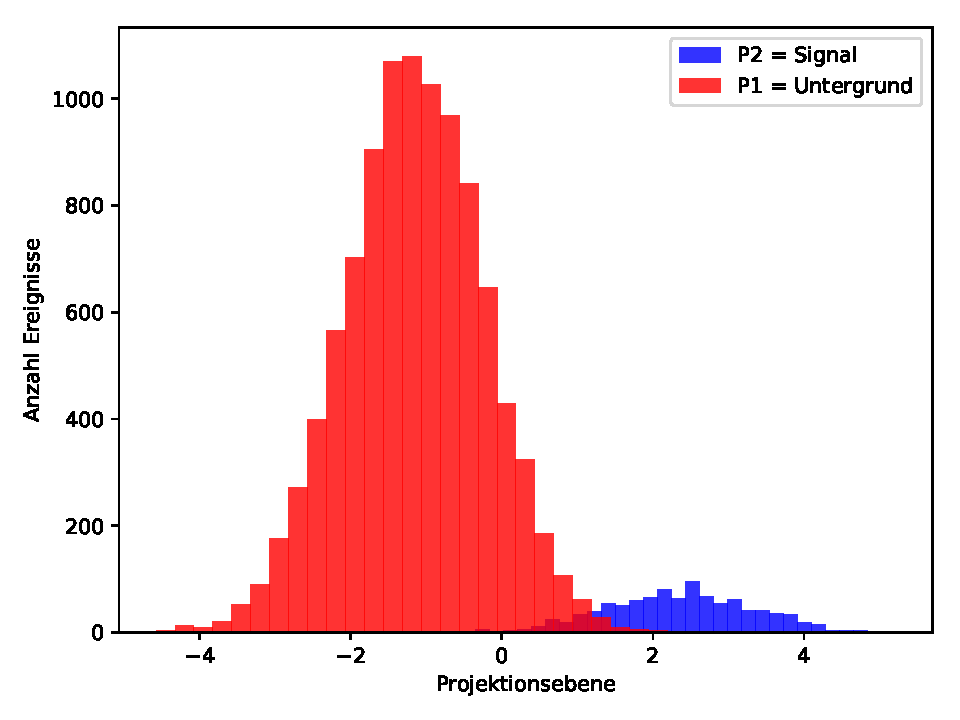
\includegraphics[scale=0.7]{Aufgabe12/Projektionen2.pdf}
  \caption{Eindimensionale Verteilung mit P2.}
  \label{abb:5}
\end{figure}

Die Effizienz und die Reinheit sind in Abbildung \ref{abb:6} zu sehen.
\begin{figure}
  \centering
  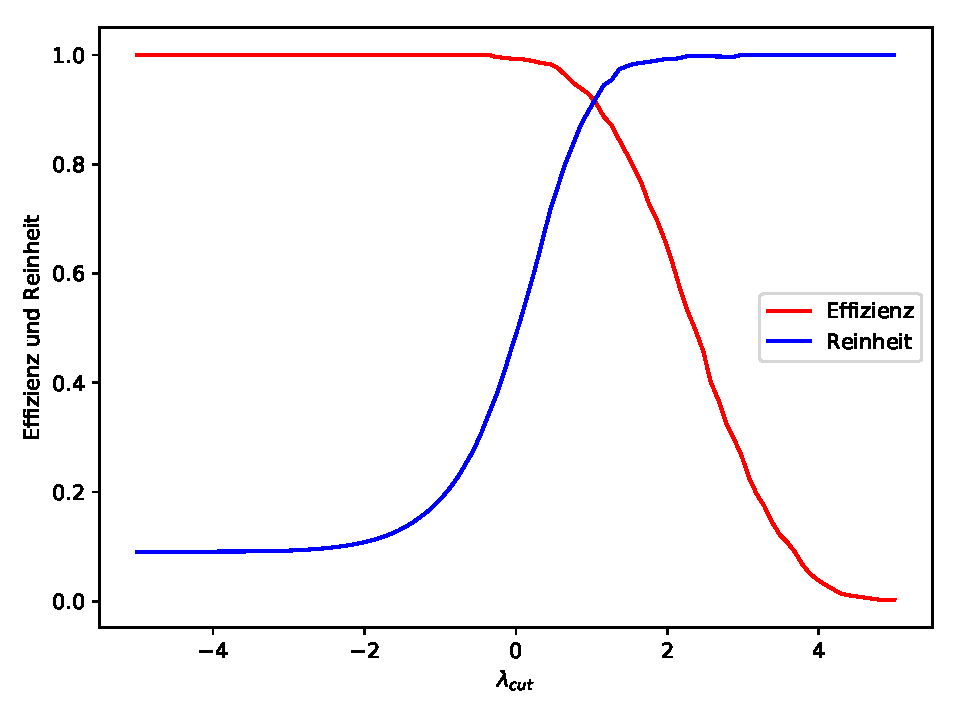
\includegraphics[scale=0.7]{Aufgabe12/EffizienzReinheit2.pdf}
  \caption{Effizienz und Reinheit der zweiten Verteilung.}
  \label{abb:6}
\end{figure}

Das Verhätnis $S/B$ in Abhängigkeit von der Cut-Stelle ist in Abbildung \ref{abb:7} dargestellt.
Das Maximum liegt bei:
\begin{equation*}
  \lambda_{\symup{cut,Verhältnis2}} \approx 2,27
\end{equation*}
\begin{figure}
  \centering
  \includegraphics[scale=0.7]{Aufgabe12/Verhältnis2.pdf}
  \caption{Verhältnis in Abhängigkeit der Cut-Stelle der zweiten Verteilung.}
  \label{abb:7}
\end{figure}

Die Signifikanzin Abhängigkeit von der Cut-Stelle ist in Abbildung \ref{abb:8} dargestellt.
Das Maximum liegt bei:
\begin{equation*}
  \lambda_{\symup{cut,Signifikanz2}} \approx 1,06
\end{equation*}
\begin{figure}
  \centering
  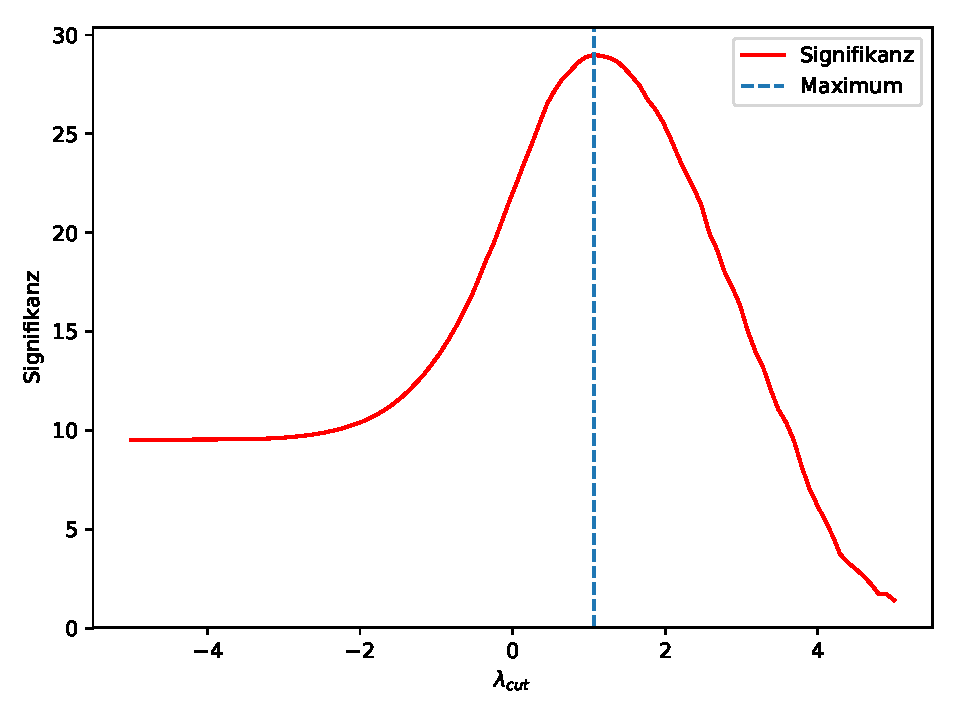
\includegraphics[scale=0.7]{Aufgabe12/Signifikanz2.pdf}
  \caption{Signifikanz in Abhängigkeit der Cut-Stelle der zweiten Verteilung.}
  \label{abb:8}
\end{figure}

Die Trennung funktioniert für kleinere oder gleichgroße Untergründe, im Bezug auf
das Signal, besser. Dies ist an den Maxima der Signifikanzkurve zu erkennen, da
das Maximum der ersten Verteilung deutlich höher liegt, als die der zweiten.
